%%%%%%%%%%%%%%%%%%%%%%%%%%%%%%%%%%%%%%%%%%%%%%%%%%%%%%%%%%%%%%%%%%%
% Lostify Final Report — aligned with implemented prototype (July 2026)
%%%%%%%%%%%%%%%%%%%%%%%%%%%%%%%%%%%%%%%%%%%%%%%%%%%%%%%%%%%%%%%%%%%
\documentclass[11pt,a4paper]{article}
\usepackage[margin=2.5cm]{geometry}
\usepackage[onehalfspacing]{setspace}
\usepackage{graphicx}
\usepackage[breaklinks=true,colorlinks=true,linkcolor=blue,urlcolor=blue,citecolor=blue]{hyperref}
\usepackage{amsmath,amsthm,amssymb}
\usepackage{icomma}
\usepackage[english]{babel}
\usepackage[T1]{fontenc}
\usepackage[locale=DE,space-before-unit=true,per-mode=symbol]{siunitx}
\usepackage{placeins}
\graphicspath{{Bilder/}}
\usepackage{tikz}
\usetikzlibrary{shapes.geometric, arrows.meta, positioning, fit, backgrounds}
\usepackage{booktabs}
\usepackage{longtable}
\usepackage{array}
\usepackage{enumitem}
\usepackage{titlesec}
\usepackage{fancyhdr}

\pagestyle{fancy}
\fancyhf{}
\fancyhead[L]{Lostify}
\fancyhead[R]{Serverless Cloud Application Automation}
\fancyfoot[C]{\thepage}
\renewcommand{\headrulewidth}{0.4pt}

\setlength{\parskip}{0.5em}
\setlength{\parindent}{0pt}
\setlength{\emergencystretch}{2em}
\sloppy
%%%%%%%%%%%%%%%%%%%%%%%%%%%%%%%%%%%%%%%%%%%%%%%%%%%%%%%%%%%%%%%%%%%
\begin{document}
%%%%%%%%%%%%%%%%%%%%%%%%%%%%%%%%%%%%%%%%%%%%%%%%%%%%%%%%%%%%%%%%%%%

\begin{titlepage}
    \centering
    \vspace*{2.0cm}
    \includegraphics[width=5cm]{logo.jpg}\\[1.8cm]
    {\LARGE Lostify\\[0.4cm]}
    {\Large Lost and Found Web App\\[1.6cm]}
    {\large
    Zain Afzal\textsuperscript{*}, Babar Ali\textsuperscript{\dag}, Muhammad Hamza Azeem\textsuperscript{\ddag}\\[0.6cm]
    Team 04\\[0.6cm]
    July 1, 2026
    }
    \vfill
    {\large Serverless Cloud Application Automation\\[0.2cm]
    Prof.\ Sashko Ristov}
    \vspace{1.5cm}

    \begin{flushleft}
        \footnotesize
        \rule{6.0cm}{0.4pt}\\[0.15cm]
        $^*$\href{mailto:zain.afzal@student.uibk.ac.at}{zain.afzal@student.uibk.ac.at}\\
        $^\dagger$\href{mailto:babar.ali@student.uibk.ac.at}{babar.ali@student.uibk.ac.at}\\
        $^\ddagger$\href{mailto:hamza.azeem@student.uibk.ac.at}{hamza.azeem@student.uibk.ac.at}\\[0.4cm]
        Repository: \href{https://github.com/Babarali2k21/Lostify}{github.com/Babarali2k21/Lostify}\\
        Live demo: \href{http://44.220.148.111:3001}{http://44.220.148.111:3001}
    \end{flushleft}
\end{titlepage}

\cleardoublepage
\thispagestyle{empty}
\renewcommand\abstractname{Abstract}
\section*{\abstractname}
\textit{
Lostify is a microservice-based lost-and-found platform where users report lost or found items,
receive automatic in-app match notifications and complete the recovery process through a claim
workflow. The system is organized around three business microservices: Item Service, Claim/Recovery
Service and Notification Service. User registration and login are implemented as application-level
JWT authentication inside Item Service---not as a separate microservice---following course guidance
on service boundaries.

The prototype uses Python FastAPI backends, SQLite databases (one per service), REST APIs,
Redis pub/sub for asynchronous events, Docker containers, AWS EC2 deployment, GitHub Actions
CI/CD and AWS Step Functions for Saga visualization and optional workflow sync. The
Claim/Recovery Service orchestrates a Saga pattern with compensation when claims are rejected.
The project demonstrates microservice decomposition, distributed transaction coordination,
event-driven notifications, API composition, container deployment, automation and evaluation
through 31 automated tests covering unit, integration, latency, fault tolerance and lead-time metrics.
}
\cleardoublepage
\tableofcontents
\thispagestyle{empty}
\cleardoublepage
\pagenumbering{arabic}
\singlespacing
\newpage

% ======================================================
\section{Introduction}
% ======================================================

People lose personal items in universities, public buildings, offices, libraries, trains, buses and
events every day. In many cases the recovery process still depends on manual communication: a
person calls an office, checks a physical lost-and-found desk, asks in a chat group or hopes that
somebody posts about the found item. This process is slow and unstructured. It is also difficult
to track whether a matching item already exists, whether the owner was notified and whether a
handover was completed.

Lostify tries to solve this problem with a digital lost-and-found platform. Users can report lost
items and found items, the system searches for possible matches and users can continue the
recovery process through the platform. A report contains information such as title, description
and item type (lost or found). If the system finds a likely pair, the owner receives an in-app
notification. The user can then submit a claim and the finder can approve or reject it.

The project is relevant for Serverless Cloud Application Automation because it has clear
business events, several bounded responsibilities and a workflow that crosses service boundaries.
Our project demonstrates microservice architecture, distributed transactions and coordination,
queries across microservices, communication and event handling, scalability, deployment,
automation and evaluation.

\subsection{Service boundary decision}

During the course, the professor advised that \textbf{User Service should not be kept as a separate
microservice}. Authentication is a cross-cutting concern that supports the domain but is not an
independent business capability. Our final architecture therefore has three business microservices:

\begin{itemize}
    \item \textbf{Item Service:} lost/found reports, keyword matching, item states, register/login/JWT.
    \item \textbf{Claim/Recovery Service:} claims, Saga orchestration, compensation, AWS Step Functions sync.
    \item \textbf{Notification Service:} Redis event consumer, in-app notification log, duplicate protection.
\end{itemize}

This split keeps item matching, claim coordination and notification handling separated while
still providing secure JWT-protected APIs across all services.

% ======================================================
\section{Solution}
% ======================================================

\subsection{Use case overview}

Lostify supports the typical lifecycle of a lost-and-found case. A user who lost an item creates a
lost-item report. A finder creates a found-item report. Each report contains a title and description.
After a report is created, the Item Service runs keyword-overlap matching logic. If a promising pair
is found, the item state changes to \texttt{MATCHED} and the Item Service publishes a \texttt{MatchFound}
event to Redis. The Notification Service consumes this event and records an in-app notification.

After a possible match is shown to the user, the user can submit a claim through the Claim/Recovery
Service. The Saga reserves the item (\texttt{MATCHED} $\rightarrow$ \texttt{RESERVED}) while the finder
reviews ownership. If the claim is accepted, the item becomes \texttt{RECOVERED}. If the claim is
rejected, compensation releases the item back to \texttt{MATCHED} so another user can claim it.

The main design scenarios implemented in the prototype are:

\begin{itemize}
    \item \textbf{Match found and owner notified:} a found item is reported, matched against open lost
    reports and the user receives an in-app notification.
    \item \textbf{Claim approved and item recovered:} the claim becomes \texttt{APPROVED} and the item
    becomes \texttt{RECOVERED}.
    \item \textbf{Claim rejected and item released:} the finder rejects the claim, the claim becomes
    \texttt{REJECTED} and the item is released again through Saga compensation.
    \item \textbf{No match found initially:} an item remains \texttt{OPEN} until a matching report is
    submitted later.
\end{itemize}

Claim cancellation before approval was discussed in the project plan but is \textbf{not implemented}
in the MVP prototype. The rejection path covers the main compensation scenario.

\subsection{Complete flow of Lostify}

The complete flow is:

\begin{enumerate}
    \item A user registers and logs in through Item Service (\texttt{POST /register}, \texttt{POST /login}).
    \item A user creates a lost or found item report (\texttt{POST /items}).
    \item The Item Service saves the item and publishes an \texttt{ItemCreated} event.
    \item The Item Service checks existing reports for keyword overlap.
    \item If a match is found: status becomes \texttt{MATCHED}, \texttt{MatchFound} is published, Notification
    Service stores the notification.
    \item If no match: status stays \texttt{OPEN}.
    \item The user submits a claim (\texttt{POST /claims} on Claim/Recovery Service).
    \item The Saga creates the claim (\texttt{PENDING}) and calls Item Service to reserve the item
    (\texttt{RESERVED}).
    \item \texttt{ClaimCreated} is published; Notification Service records it.
    \item If approved: item \texttt{RECOVERED}, events \texttt{ClaimApproved} and \texttt{ItemRecovered}.
    \item If rejected: compensation releases item to \texttt{MATCHED}, event \texttt{ClaimRejected}.
\end{enumerate}

The verified happy-path event sequence from integration tests is:
\texttt{ItemCreated} $\rightarrow$ \texttt{ItemCreated} $\rightarrow$ \texttt{MatchFound} $\rightarrow$
\texttt{ClaimCreated} $\rightarrow$ \texttt{ClaimApproved} $\rightarrow$ \texttt{ItemRecovered}.

\subsection{Project objectives and requirements}

The project objectives are a microservice-based application with distributed transactions,
queries across microservices, data management across services, communication and event handling,
deployment, automation and evaluation.

\begingroup
\small
\renewcommand{\arraystretch}{1.35}
\setlength{\tabcolsep}{6pt}

\begin{longtable}{@{}
>{\raggedright\arraybackslash}p{3.0cm}
>{\raggedright\arraybackslash}p{7.4cm}
>{\raggedright\arraybackslash}p{4.0cm}
@{}}
\caption{Project requirements and objectives}
\label{tab:requirements} \\
\toprule
\textbf{Requirement} & \textbf{Details} & \textbf{Objective} \\
\midrule
\endfirsthead

\multicolumn{3}{c}{\tablename\ \thetable\ -- continued} \\
\toprule
\textbf{Requirement} & \textbf{Details} & \textbf{Objective} \\
\midrule
\endhead

Item reports &
Item Service handles lost/found reports, keyword matching and item states
(\texttt{OPEN}, \texttt{MATCHED}, \texttt{RESERVED}, \texttt{RECOVERED}). Auth (register/login/JWT) is embedded here. &
Business-capability decomposition. \\[0.45em]

Claim and recovery &
Claim/Recovery Service handles claim creation, claim states, recovery decisions, Saga coordination and compensation. &
Distributed workflow and Saga coordination. \\[0.45em]

Notifications &
Notification Service consumes Redis pub/sub events and stores in-app notifications with \texttt{eventId} deduplication. &
Event-driven architecture and asynchronous communication. \\[0.45em]

Separate databases &
Each service owns its own SQLite database (\texttt{item.db}, \texttt{claim.db}, \texttt{notification.db}). &
Data ownership and loose coupling. \\[0.45em]

Cross-service workflow &
Claim/recovery workflow modeled as ClaimRecoverySaga with compensation; mirrored in AWS Step Functions. &
Distributed transactions and coordination. \\[0.45em]

Queries across services &
React dashboard uses API composition across Item, Claim/Recovery and Notification services. &
Cross-service queries. \\[0.45em]

Cloud deployment &
Services packaged as Docker containers on AWS EC2. Redis internal. Step Functions in \texttt{eu-central-1}. &
Container deployment and cloud/serverless workflow. \\[0.45em]

Automation &
GitHub Actions: pytest, Docker build, rsync deploy to EC2, health checks. &
CI/CD and lead-time evaluation. \\[0.45em]

Evaluation &
31 automated tests plus demo scripts, latency measurement and evaluation report generator. &
Automation and evaluation. \\

\bottomrule
\end{longtable}
\endgroup

The functional requirements are item reports, automatic matching, in-app notifications and
ownership claims. The non-functional requirements are loose coupling, scalability, consistency
and maintainability.

\newpage

\subsection{Project implementation}

The final design is based on \textbf{three microservices} and a React frontend. The Item Service
handles authentication, item reports, matching and item status. The Claim/Recovery Service
handles claims, Saga orchestration and AWS Step Functions integration. The Notification Service
listens to Redis events and stores processed notifications.

\begin{table}[h]
\centering
\small
\renewcommand{\arraystretch}{1.3}
\begin{tabular}{@{}lll@{}}
\toprule
\textbf{Layer} & \textbf{Technology} & \textbf{Notes} \\
\midrule
Frontend & React 18 + Vite + nginx & Port 3001; proxies \texttt{/api/item/*}, \texttt{/api/claim/*}, \texttt{/api/notif/*} \\
Backend & Python 3.12 + FastAPI & Three independent services \\
Databases & SQLite per service & PostgreSQL via RDS documented as upgrade path \\
Event bus & Redis 7 pub/sub & Channel \texttt{lostify:events} \\
Containers & Docker Compose & Local + \texttt{docker-compose.prod.yml} on EC2 \\
Cloud & AWS EC2 (Ubuntu 24.04) & Public demo at \texttt{44.220.148.111:3001} \\
Workflow & AWS Step Functions + 5 Lambdas & Region \texttt{eu-central-1} \\
CI/CD & GitHub Actions & \texttt{ci.yml} + \texttt{deploy.yml} \\
\bottomrule
\end{tabular}
\caption{Implementation stack}
\label{tab:stack}
\end{table}

\begin{figure}[h]
\centering
\resizebox{\textwidth}{!}{%
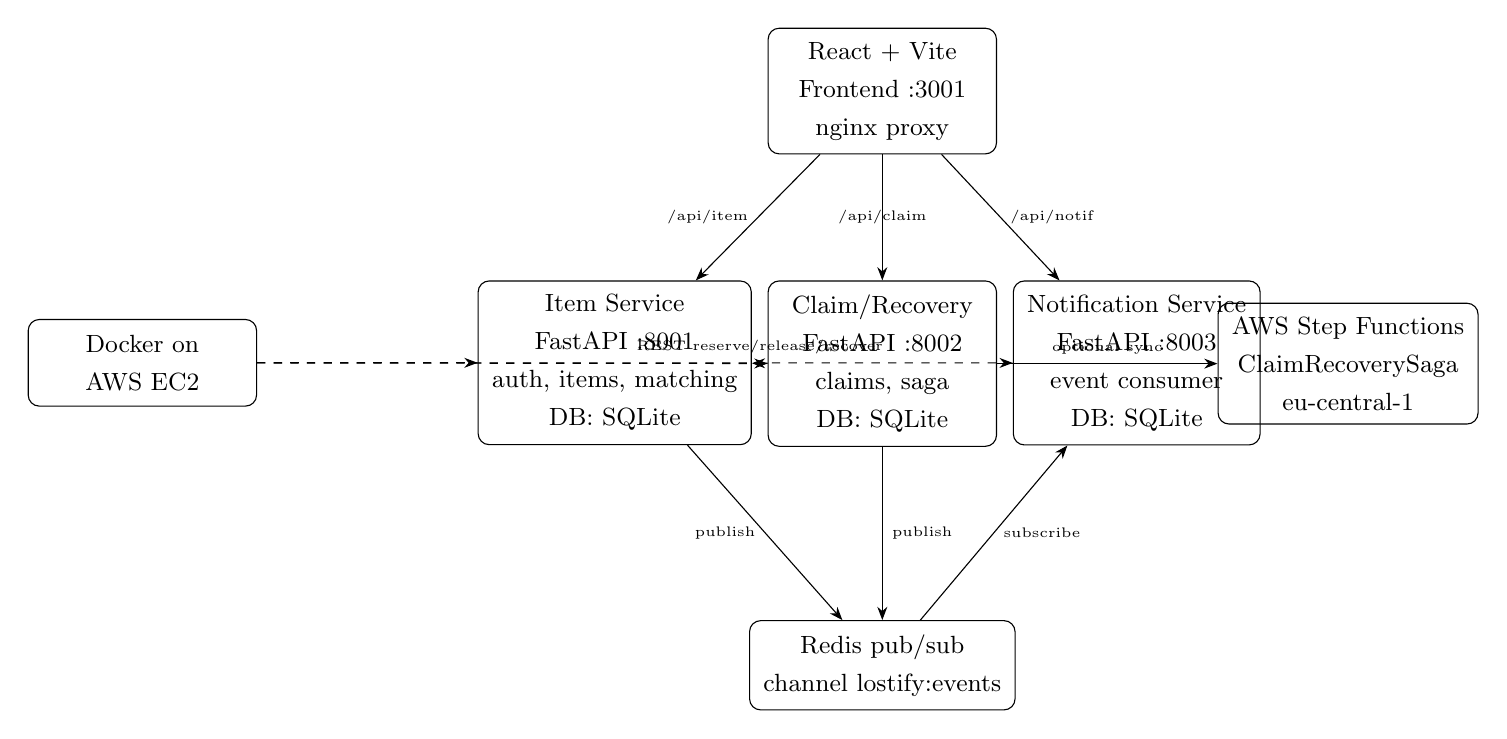
\begin{tikzpicture}[
    box/.style={
        draw,
        rounded corners,
        align=center,
        font=\small,
        minimum width=2.9cm,
        minimum height=1.1cm,
        inner sep=5pt
    },
    svc/.style={box},
    ext/.style={box},
    client/.style={box},
    >=Stealth,
    node distance=1.5cm and 2.0cm
]

\node[client] (web) {React + Vite\\Frontend :3001\\nginx proxy};

\node[svc, below left=1.6cm and 0.2cm of web] (item)
{Item Service\\FastAPI :8001\\auth, items, matching\\DB: SQLite};

\node[svc, below=1.6cm of web] (claim)
{Claim/Recovery\\FastAPI :8002\\claims, saga\\DB: SQLite};

\node[svc, below right=1.6cm and 0.2cm of web] (notif)
{Notification Service\\FastAPI :8003\\event consumer\\DB: SQLite};

\node[ext, below=2.2cm of claim] (redis)
{Redis pub/sub\\channel lostify:events};

\node[ext, right=2.8cm of claim] (sf)
{AWS Step Functions\\ClaimRecoverySaga\\eu-central-1};

\node[ext, left=2.8cm of item] (ec2)
{Docker on\\AWS EC2};

\draw[->] (web) -- node[left,font=\tiny]{/api/item} (item);
\draw[->] (web) -- node[font=\tiny]{/api/claim} (claim);
\draw[->] (web) -- node[right,font=\tiny]{/api/notif} (notif);

\draw[->] (item) -- node[left,font=\tiny]{publish} (redis);
\draw[->] (claim) -- node[right,font=\tiny]{publish} (redis);
\draw[->] (redis) -- node[right,font=\tiny]{subscribe} (notif);

\draw[->] (claim) -- node[above,font=\tiny]{REST reserve/release/recover} (item);
\draw[->] (claim) -- node[above,font=\tiny]{optional sync} (sf);

\draw[dashed,->] (ec2) -- (item);
\draw[dashed,->] (ec2) -- (claim);
\draw[dashed,->] (ec2) -- (notif);

\end{tikzpicture}
}
\caption{Lostify architecture with three microservices, Redis events and AWS Step Functions}
\label{fig:architecture}
\end{figure}

The development process followed the project milestones. During implementation the team worked on
Item Service, Claim/Recovery Service, Notification Service, matching logic, Redis event flow,
Step Functions workflow, React frontend, EC2 deployment, GitHub Actions CI/CD and end-to-end testing.

\subsection{Main implementation innovation}

The main idea of our implementation is to combine automatic item matching with a controlled
recovery process governed by a Saga. Lostify compares lost and found reports, detects possible
matches, creates in-app notifications and then guides the item through claim and recovery.

An important decision was to \textbf{separate item logic from claim and recovery logic}. Matching
stays in the Item Service because it directly depends on item data. The claim and recovery
workflow is handled by the Claim/Recovery Service because claims have their own states and
compensation rules. This makes the Saga clearer and gives the workflow its own service boundary.

A third important part is the \textbf{hybrid Saga model}. Locally, \texttt{claim-recovery-service/app/saga.py}
orchestrates the real demo and calls Item Service REST endpoints. On AWS, Step Functions provides
a visual orchestration graph with the same logical steps (CreateClaim $\rightarrow$ ReserveItem $\rightarrow$
Choice $\rightarrow$ RecoverItem or ReleaseItem). The frontend Saga panel can show both local saga state
and optional AWS execution status.

\subsection{Implementation challenges}

\subsubsection{Development challenges}

The first challenge was deciding how to split the system. We defined three business microservices
and placed JWT authentication inside Item Service rather than creating a fourth service. The second
challenge was designing stable Redis event payloads with \texttt{eventId}, \texttt{eventType},
\texttt{payload} and \texttt{timestamp}. The third challenge was Saga coordination: Claim/Recovery
Service must call Item Service atomically per step with clear failure handling.

\subsubsection{Evaluation challenges}

The evaluation is harder than evaluating a single REST API because parts of the system run
asynchronously. A user may receive a quick response after submitting an item while notification
handling continues in the background. Therefore the evaluation must measure both synchronous
request response time and end-to-end event latency. Results can differ between local Docker Compose
and AWS EC2 deployment.

\subsubsection{Team work challenges}

The main team challenge was coordination across service interfaces. Each team member had a
service responsibility but the services still needed to agree on API and event contracts. This was
especially important between Item Service (\texttt{/items/\{id\}/reserve|release|recover}) and
Claim/Recovery Service.

\subsubsection{Other challenges}

The cloud setup required balancing learning goals with prototype simplicity. Docker and EC2 kept
deployment manageable. AWS Step Functions helped visualize the Saga. GitHub secrets
(\texttt{EC2\_HOST}, \texttt{EC2\_USER}, \texttt{EC2\_SSH\_KEY}) and IMDSv2 hop limit configuration
were needed for automated deploy and Step Functions sync from EC2 containers.

% ======================================================
\section{Core techniques and implementation decisions}
% ======================================================

\subsection{Microservice architecture}

Lostify follows the microservice architecture pattern by decomposing the application around
business responsibilities:

\begin{itemize}
    \item \textbf{Item Service:} owns lost/found item reports, keyword matching, item states and JWT auth.
    \item \textbf{Claim/Recovery Service:} owns claims, claim states, Saga orchestration and Step Functions sync.
    \item \textbf{Notification Service:} owns in-app notification records and processed Redis event IDs.
\end{itemize}

Each service has its own SQLite database and the services do not share tables. This keeps data
separate and reduces tight coupling. The downside is that queries and transactions become more
difficult because the data is not stored in one shared database. Lostify uses API composition,
Redis events and Saga-style compensation to handle this.

\subsection{Transactions and coordination}

The main distributed workflow is the claim and recovery process. Since services have separate
databases, we cannot handle all steps with one database transaction. Instead, the Claim/Recovery
Service orchestrates the workflow step by step. If a claim is rejected, compensation releases the
item through \texttt{POST /items/\{id\}/release} on Item Service.

\textbf{Item state machine:}
\texttt{OPEN} $\rightarrow$ \texttt{MATCHED} $\rightarrow$ \texttt{RESERVED} $\rightarrow$ \texttt{RECOVERED};
reject path: \texttt{RESERVED} $\rightarrow$ \texttt{MATCHED}.

\textbf{Claim state machine:}
\texttt{PENDING} $\rightarrow$ \texttt{APPROVED} or \texttt{REJECTED}.

\newpage

\begin{figure}[h]
\centering
\resizebox{\textwidth}{!}{%
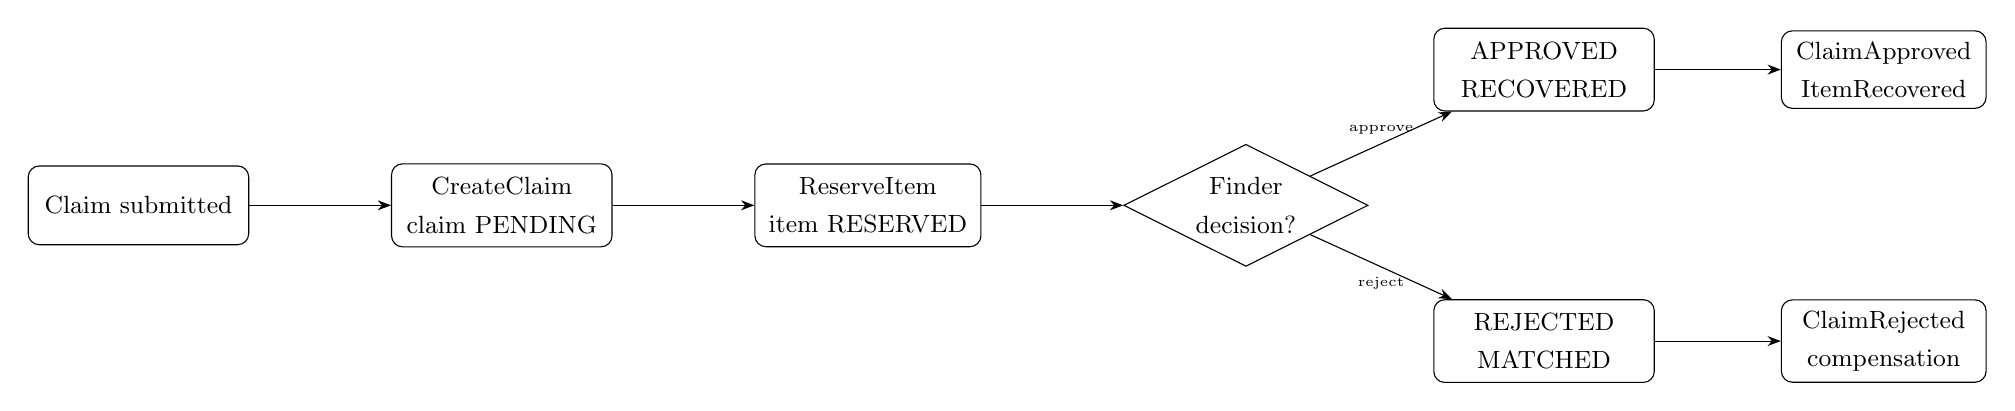
\begin{tikzpicture}[
    node distance=1.0cm and 1.8cm,
    state/.style={
        draw,
        rounded corners,
        align=center,
        font=\small,
        minimum width=2.8cm,
        minimum height=1.0cm,
        inner sep=5pt
    },
    decision/.style={
        draw,
        diamond,
        aspect=2,
        align=center,
        font=\small,
        inner sep=2pt
    },
    notif/.style={
        draw,
        rounded corners,
        align=center,
        font=\small,
        minimum width=2.6cm,
        minimum height=0.9cm,
        inner sep=4pt
    },
    >=Stealth
]

\node[state] (submit) {Claim submitted};

\node[state, right=of submit] (create)
{CreateClaim\\claim PENDING};

\node[state, right=of create] (reserve)
{ReserveItem\\item RESERVED};

\node[decision, right=of reserve] (decide)
{Finder\\decision?};

\node[state, above right=0.8cm and 1.6cm of decide] (approved)
{APPROVED\\RECOVERED};

\node[state, below right=0.8cm and 1.6cm of decide] (rejected)
{REJECTED\\MATCHED};

\node[notif, right=1.6cm of approved] (notifyok)
{ClaimApproved\\ItemRecovered};

\node[notif, right=1.6cm of rejected] (notifyno)
{ClaimRejected\\compensation};

\draw[->] (submit) -- (create);
\draw[->] (create) -- (reserve);
\draw[->] (reserve) -- (decide);
\draw[->] (decide) -- node[above,font=\tiny]{approve} (approved);
\draw[->] (decide) -- node[below,font=\tiny]{reject} (rejected);
\draw[->] (approved) -- (notifyok);
\draw[->] (rejected) -- (notifyno);

\end{tikzpicture}
}
\caption{Claim and recovery Saga: happy path and compensation path}
\label{fig:saga}
\end{figure}

The happy path is:

\begin{enumerate}
    \item The user submits a claim for a matched item through the frontend.
    \item Claim/Recovery Service creates a claim in \texttt{PENDING} state.
    \item The Saga calls Item Service to reserve the item (\texttt{RESERVED}).
    \item \texttt{ClaimCreated} is published to Redis.
    \item The finder approves; Item Service marks the item \texttt{RECOVERED}.
    \item Events \texttt{ClaimApproved} and \texttt{ItemRecovered} are published.
    \item Notification Service consumes the events and records notifications.
\end{enumerate}

The rejection path releases the item back to \texttt{MATCHED} and publishes \texttt{ClaimRejected}.
Compensation is not a database rollback---it is a new forward update that undoes the reserve step.

\subsection{Queries across microservices}

Lostify has queries that span multiple services. The React dashboard needs item status from Item
Service, processed events from Notification Service and saga status from Claim/Recovery Service.
Since each service owns its own database, the frontend uses \textbf{API composition}:

\begin{itemize}
    \item \texttt{GET /items} --- Item Service
    \item \texttt{GET /events/processed} --- Notification Service
    \item \texttt{GET /claims/\{id\}/saga} --- Claim/Recovery Service
\end{itemize}

Pull synchronization: the dashboard fetches current state on refresh.
Push synchronization: \texttt{MatchFound} and claim events update Notification Service asynchronously via Redis.

\subsection{Communication and event handling}

Lostify uses REST for synchronous operations (create item, submit claim, approve/reject) and
Redis pub/sub for asynchronous notifications on channel \texttt{lostify:events}.

Implemented event types: \texttt{ItemCreated}, \texttt{MatchFound}, \texttt{ClaimCreated},
\texttt{ClaimApproved}, \texttt{ClaimRejected}, \texttt{ItemRecovered}.

Each event contains \texttt{eventId}, \texttt{eventType}, \texttt{timestamp} and \texttt{payload}.
The Notification Service stores processed \texttt{eventId} values to prevent duplicate notifications---
verified by unit tests, fault-tolerance tests and \texttt{scripts/test\_duplicate\_events.py}.

\subsection{Scalability and serverless deployment}

Lostify uses Docker containers on AWS EC2 (\texttt{t3.small}, Ubuntu 24.04). Redis is not exposed
publicly in production compose. Five mock Lambda functions and a Step Functions state machine
(\texttt{aws/step-functions/claim-recovery-saga.asl.json}) mirror the Saga for presentation.

\textbf{GitHub Actions pipeline:}
\begin{itemize}
    \item \texttt{ci.yml}: unit tests $\rightarrow$ integration tests (Docker) $\rightarrow$ Docker build.
    \item \texttt{deploy.yml}: pre-deploy tests $\rightarrow$ rsync to EC2 $\rightarrow$
    \texttt{docker compose up --build} $\rightarrow$ health check on all three services.
\end{itemize}

The deploy job uses \texttt{environment: production} so the repository Deployments sidebar reflects status.
Measured lead time from commit to deployed EC2: approximately \textbf{3--5 minutes}.

\subsection{Portability and interoperability}

Portable elements: HTTP/REST, JSON, Docker, SQLite (dev) with PostgreSQL upgrade path, Redis pub/sub.
AWS-specific elements: Step Functions, EC2 security groups, Lambda ARNs in ASL.
Event format abstraction in \texttt{shared/events/} allows swapping Redis for another broker if the envelope stays stable.

\newpage

% ======================================================
\section{Evaluation}
% ======================================================

\subsection{Evaluation methodology}

The evaluation checks whether the main parts of Lostify work correctly and whether the system
behaves well under normal conditions. We evaluate services separately, then test the complete
flow with Docker Compose and on AWS EC2. The evaluation covers performance, event latency,
fault handling and deployment automation.

\begingroup
\small
\renewcommand{\arraystretch}{1.45}
\setlength{\tabcolsep}{7pt}

\begin{longtable}{
@{}
>{\raggedright\arraybackslash}p{3.0cm}
>{\raggedright\arraybackslash}p{5.8cm}
>{\raggedright\arraybackslash}p{5.0cm}
@{}
}
\caption{Evaluation methodology for Lostify}
\label{tab:evaluation-methodology} \\

\toprule
\textbf{Evaluation part} & \textbf{Method} & \textbf{What it shows} \\
\midrule
\endfirsthead

\multicolumn{3}{c}{\tablename\ \thetable\ -- continued} \\
\toprule
\textbf{Evaluation part} & \textbf{Method} & \textbf{What it shows} \\
\midrule
\endhead

Unit tests &
pytest on events, deduplication, saga logic and Step Functions client (22 tests, no Docker). &
Local correctness of domain logic and saga rules. \\[0.6em]

Integration tests &
Docker Compose stack; E2E happy path and reject compensation (2 tests). &
Service contracts and end-to-end workflow. \\[0.6em]

Fault-tolerance tests &
Duplicate events, invalid transitions, auth errors, double approve (5 tests). &
Idempotency, authorization and compensation. \\[0.6em]

Event latency test &
Measure \texttt{MatchFound} and \texttt{ClaimCreated} async latency (2 tests + script). &
Delay caused by Redis pub/sub processing. \\[0.6em]

Demo scripts &
\texttt{demo.sh}, \texttt{demo\_reject.sh}, \texttt{demo\_saga.sh}, duplicate event script. &
Manual demonstration evidence for evaluation. \\[0.6em]

Lead-time test &
GitHub Actions CI and Deploy workflow duration. &
Automation quality and deployment speed. \\

\bottomrule
\end{longtable}
\endgroup

\textbf{Total automated tests: 31} (22 unit + 9 integration/fault/latency).

Run locally:
\begin{verbatim}
docker compose up --build -d
./scripts/run-all-tests.sh
./scripts/evaluation-report.sh
\end{verbatim}

\subsection{Functional evaluation results}

\begingroup
\small
\renewcommand{\arraystretch}{1.35}
\setlength{\tabcolsep}{6pt}

\begin{longtable}{@{}
>{\raggedright\arraybackslash}p{4.5cm}
>{\raggedright\arraybackslash}p{3.5cm}
>{\raggedright\arraybackslash}p{5.5cm}
@{}}
\caption{Functional test scenarios}
\label{tab:functional} \\
\toprule
\textbf{Scenario} & \textbf{Expected} & \textbf{Verified by} \\
\midrule
\endfirsthead
\multicolumn{3}{c}{\tablename\ \thetable\ -- continued} \\
\toprule
\textbf{Scenario} & \textbf{Expected} & \textbf{Verified by} \\
\midrule
\endhead

Register + login & JWT returned & \texttt{test\_full\_demo\_flow} \\
Create lost + found items & Items stored & \texttt{test\_full\_demo\_flow} \\
Keyword matching & \texttt{MATCHED} + \texttt{MatchFound} & \texttt{test\_full\_demo\_flow} \\
Submit claim & \texttt{RESERVED} item & \texttt{test\_submit\_claim\_reserves\_item} \\
Approve claim & \texttt{RECOVERED}, saga completed & \texttt{test\_approve\_completes\_saga} \\
Reject claim & \texttt{MATCHED}, compensated & \texttt{test\_reject\_compensates\_*} \\
Claim on OPEN item & HTTP 400 & \texttt{test\_cannot\_claim\_open\_item} \\
Double approve & HTTP 400 & \texttt{test\_cannot\_approve\_twice} \\
Wrong user approves & HTTP 403 & \texttt{test\_wrong\_user\_cannot\_approve} \\
Duplicate Redis event & Ignored & \texttt{test\_duplicate\_event\_*} \\

\bottomrule
\end{longtable}
\endgroup

\subsection{Results and interpretation}

\begingroup
\small
\renewcommand{\arraystretch}{1.4}
\setlength{\tabcolsep}{6pt}

\begin{longtable}{
@{}
>{\raggedright\arraybackslash}p{4.1cm}
>{\raggedright\arraybackslash}p{2.8cm}
>{\raggedright\arraybackslash}p{6.0cm}
@{}
}
\caption{Evaluation results for Lostify (measured on prototype)}
\label{tab:results} \\

\toprule
\textbf{Metric} & \textbf{Value} & \textbf{Meaning} \\
\midrule
\endfirsthead

\multicolumn{3}{c}{\tablename\ \thetable\ -- continued} \\
\toprule
\textbf{Metric} & \textbf{Value} & \textbf{Meaning} \\
\midrule
\endhead

Automated test count &
\texttt{31} &
Full pytest suite covering unit, integration, fault and latency. \\[0.6em]

Unit test duration &
\texttt{$\sim$30 s} &
Fast feedback without Docker. \\[0.6em]

MatchFound event latency (local) &
\texttt{50--500 ms} &
Typical async path via Redis pub/sub. \\[0.6em]

ClaimCreated event latency (local) &
\texttt{50--500 ms} &
Saga publish-to-notification delay. \\[0.6em]

Latency test threshold (CI) &
\texttt{< 5000 ms} &
Generous bound for CI and EC2 variance. \\[0.6em]

Duplicate event handling &
\texttt{PASS} &
Live script and automated tests confirm deduplication. \\[0.6em]

CI workflow duration &
\texttt{$\sim$2--3 min} &
Unit + integration + Docker build on GitHub Actions. \\[0.6em]

Deploy workflow duration &
\texttt{$\sim$1 min} &
rsync, rebuild and health check on EC2. \\[0.6em]

Commit-to-production lead time &
\texttt{3--5 min} &
Combined CI + deploy pipeline. \\[0.6em]

Live EC2 health &
\texttt{3/3 OK} &
Item, Claim/Recovery and Notification via frontend proxy. \\

\bottomrule
\end{longtable}
\endgroup

The results show that the main user actions and Saga paths work correctly under automated tests.
Asynchronous notification adds tens to hundreds of milliseconds locally, which is acceptable because
it does not block the initial HTTP response. The CI/CD pipeline provides reproducible deployment
to EC2 with minimal manual steps (GitHub secrets configured once).

\subsection{Demo checklist for live evaluation}

\begin{itemize}
    \item Open \url{http://44.220.148.111:3001} --- register users, create lost + found items.
    \item Confirm \texttt{MatchFound} in events panel.
    \item Submit claim $\rightarrow$ saga \texttt{AWAITING\_DECISION}, item \texttt{RESERVED}.
    \item Approve $\rightarrow$ \texttt{RECOVERED}; reject $\rightarrow$ compensation to \texttt{MATCHED}.
    \item AWS Console: Step Functions graph --- run APPROVED and REJECTED executions.
    \item GitHub Actions: green CI and Deploy workflows on \texttt{main}.
    \item Run \texttt{./scripts/evaluation-report.sh} for timestamped summary.
\end{itemize}

\newpage

% ======================================================
\section{Discussion}
% ======================================================

\subsection{Threats to validity}

\begin{itemize}
    \item \textbf{Prototype scale:} tests use controlled descriptions; real user data may reduce matching accuracy.
    \item \textbf{Local versus cloud:} Docker Compose latency differs from EC2 network behavior.
    \item \textbf{Simplified matching:} keyword overlap is transparent but not production-grade.
    \item \textbf{Limited failure injection:} not all distributed failure combinations are tested.
    \item \textbf{SQLite in MVP:} not the same concurrency profile as PostgreSQL on RDS.
\end{itemize}

\subsection{Project solution limitations}

Lostify is a working prototype but not a production system. It lacks strong identity verification,
claim cancellation endpoint, email delivery (console-log notifications only), and admin dispute workflow.
SQLite is used instead of PostgreSQL in the MVP. Step Functions Lambdas are mock handlers for
visualization; the local Saga drives the live demo.

\subsection{Self reflection}

\begingroup
\small
\renewcommand{\arraystretch}{1.45}
\setlength{\tabcolsep}{7pt}

\begin{longtable}{
@{}
>{\raggedright\arraybackslash}p{2.9cm}
>{\raggedright\arraybackslash}p{5.5cm}
>{\raggedright\arraybackslash}p{5.3cm}
@{}
}
\caption{Individual reflection and main contributions}
\label{tab:reflection} \\

\toprule
\textbf{Student} & \textbf{Main contribution} & \textbf{Reflection} \\
\midrule
\endfirsthead

\multicolumn{3}{c}{\tablename\ \thetable\ -- continued} \\
\toprule
\textbf{Student} & \textbf{Main contribution} & \textbf{Reflection} \\
\midrule
\endhead

Zain Afzal &
Notification Service, Redis event handling, in-app notifications, duplicate event handling and integration testing. &
I learned that notifications need \texttt{eventId} deduplication. Next time I would define event contracts earlier. \\[0.8em]

Babar Ali &
Claim/Recovery Service, Saga orchestration, AWS Step Functions, EC2 deployment and GitHub Actions CI/CD. &
I learned that a Saga needs explicit failure paths and compensation. Next time I would design the state machine diagram before coding. \\[0.8em]

Muhammad Hamza Azeem &
Item Service, item creation, matching logic, item status updates, auth merge and workflow tests. &
I learned that keeping matching inside Item Service simplified the prototype. In a larger system I would separate matching only if data volume demands it. \\

\bottomrule
\end{longtable}
\endgroup

% ======================================================
\section{Conclusion and future work}
% ======================================================

Lostify demonstrates how a lost-and-found use case can be built with three business microservices,
event-driven notifications and Saga-based claim recovery with compensation. Authentication is
correctly embedded in Item Service rather than as a separate microservice. The system uses REST
for synchronous requests, Redis pub/sub for asynchronous events, Docker on AWS EC2 for deployment
and GitHub Actions for automated test-and-deploy pipelines. AWS Step Functions provides a visual
mirror of the same Saga workflow.

Future work includes PostgreSQL on RDS, email via SES, image storage on S3, claim cancellation,
better matching, live Lambda handlers calling EC2 services, and stronger privacy controls.

\section*{Declaration}

AI tools (including Cursor) were used to help with wording, LaTeX formatting, debugging CI/CD
issues and aligning documentation with the implemented prototype. All architecture decisions,
implementation and evaluation were performed by the team.

\end{document}
